\documentclass{article}

\usepackage{graphicx}

\begin{document}
	\begin{titlepage}
	
	\centering	
		\huge \textbf{Morphological Operations} \\
	\large
		Authors: Dheeraj Kamath, Niharika Jayanthi \\
		June 1, 2015 \\
		Mentor: Sanam Shakya \\
	
		
		\end{titlepage}
\begin{flushleft}
	\huge	\textbf{Introduction} \\
	 \large 
	\indent	Morphological operations in image processing are a set of operations that are applied on images to process them. These operations are commonly used on binary images (On grayscale images, these operators can reduce noise or brighten the image). Another input that is required to perform these operations is structuring elements. Structuring elements are used to probe a binary image. These probes are themselves binary images shaped in rectangles, ellipses, diamonds, crosses or other (possibly arbitrary) shapes. \\
	
	\huge \textbf{Structuring Elements} \\
	\large
	Structuring elements are small binary images that are represented by a special matrix format. Following are matrix formats of some shapes- \\
	
	\begin{itemize}
		\item Rectangle \\ 
		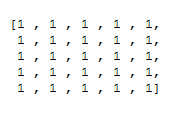
\includegraphics{Rectangle.png} \\
		\item Diamond \\ 
		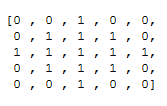
\includegraphics{Diamond.png} \\
			\item Ellipse \\ 
			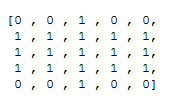
\includegraphics{Ellipse.png} \\ \hspace{0.5pt} \\
			\hspace{0.5pt} \\
			\hspace{0.5pt} \\
			\item Cross \\
			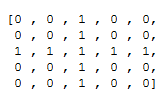
\includegraphics{Cross.png} \\
	\end{itemize}
	\huge \textbf{Morphological Operations}	\\
	\large As discussed above, morphological operations are a set of techniques used for image processing. Following are two basic morphological operations:
	
	\huge \textbf{Erosion} \\
	\large
	Erosion is a basic morphological operation applied on binary (or grayscale) images that erodes away the boundaries of regions of foreground pixels(i.e. white pixels). Thus, any holes within those areas become larger.
	\\ Erosion can be mathematically defined as- If X denotes total set of points on the image, S denotes the set of points on the structuring element and Sx denotes translation of T such that its origin is at x, then erosion of X by S is set of all points x such that Sx is a subset of X. \\
	The function used for erosion is- cv2.erode(img, kernel, iterations)  where img : \ \ \ \ \ \ \ \  Image to be eroded\\
	\ \ \ \ \ \ \ \ \        kernel : \ \ \ \ \ Structuring element used  \\
	\ \ \ \ \ \ \ \ \      iterations : Number of iterations to be applied \\
	Example - \\
	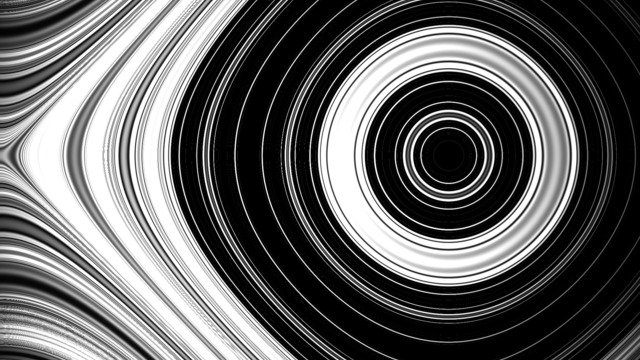
\includegraphics[width = 75mm]{music.jpg} \\
	\small Sample image \\
	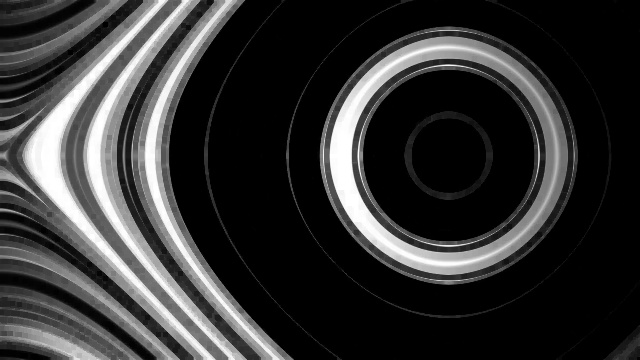
\includegraphics[width = 75mm]{Eroded.jpg} \\
	\small Eroded image \\
	\huge \textbf{Dilation} \\
	\large
	Dilation is a basic morphological operation applied on binary (or grayscale) images that increases the size of the foreground pixels(i.e. white pixels). Thus, any holes in the image shrink whereas the boundaries of image expand. \\
	Dilation can be mathematically defined as- If X denoes total set of points in an image, S denotes set of all points on the structuring element and Sx denotes translation of S such that its origin is at x, then dilation of X by S is a set of all point x where the intersection of X and Sx is non-empty. \\
	The function used for dilation is- cv2.dilate(img, kernel, iterations)  where img: \ \ \ \ \ \ \ \ \   Image to be dilated\\
	\ \ \ \ \ \ \ \ \        kernel : \ \ \ \ \ Structuring element used  \\
	\ \ \ \ \ \ \ \ \      iterations : Number of iterations to be applied \\
	Example - \\
		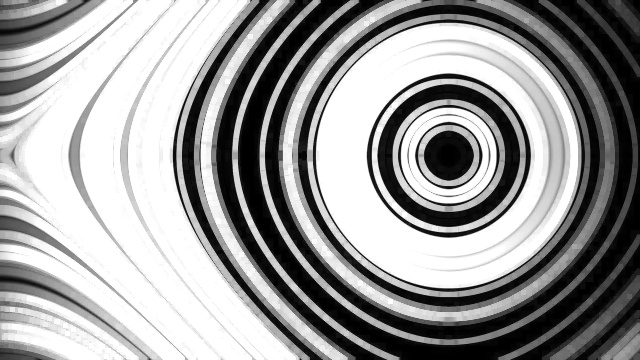
\includegraphics[width = 75mm]{Dilated.jpg} \\
		\small Diated image \\
		
	
	
\end{flushleft}
		
\end{document}